\lab{Applications}{Julia Sets and Basins of Attraction}{Julia Sets}

\objective{Understand definition of basin of attraction.  Basic understanding of Julia Sets.}

%\begin{itemize}
%\item Recall Newton's method
%\item Different seed values for Newton yield different roots.
%\item Definition of basin of attraction.
%\end{itemize}

Recall Newton's method for finding the roots of a function in one variable.  Given the function $f$ and a seed value $x_0$, we can iteratively find a root:
\[
x_{n+1} = x_n - \frac{f(x_n)}{f'(x_n)}
\]
We have shown in previous sections that this method will converge very quickly to a root.  For example, given
\[
f(x) = x^2 + x -2
\]
and a seed value of $x_0 = 4$, after only 4 iterations we are about as close to the true root at $1$ as we would like.  What happens, however, when we choose a different seed value, say $x_0 = -4$?  Going through the Newton iterations, we notice that we quickly converge to the other root of the function, $-2$.

\begin{figure}
\begin{center}
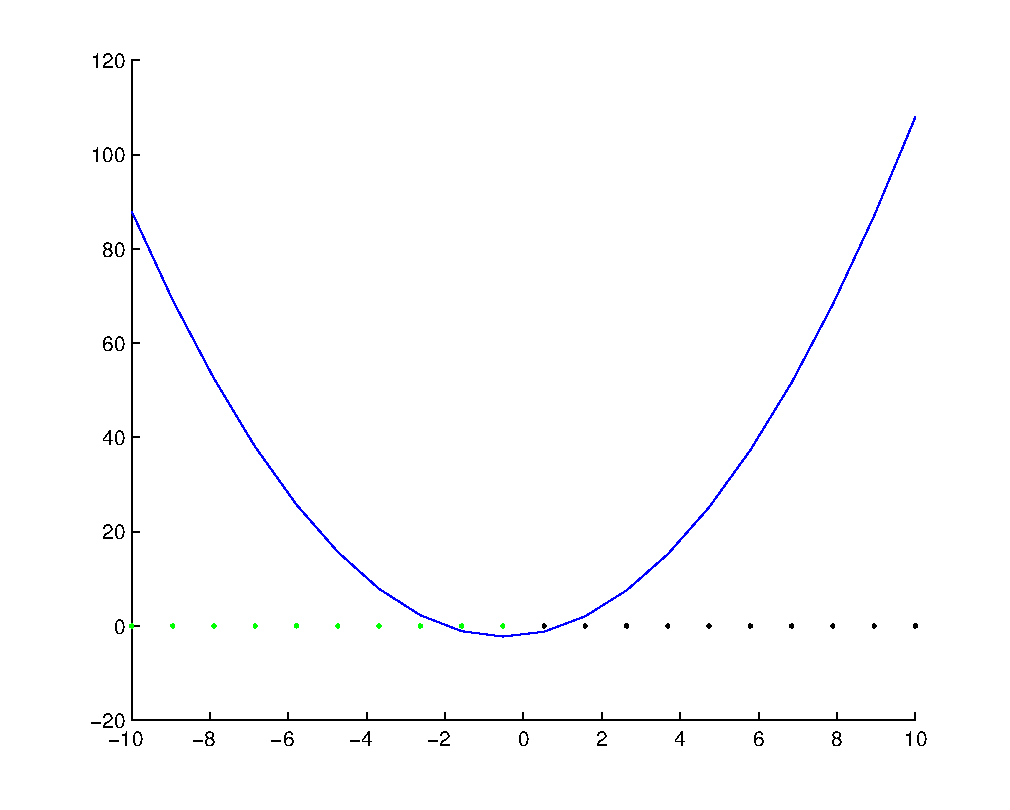
\includegraphics[scale=0.5]{basins1}
\caption{The plot of $f(x) = x^2 + x - 2$ along with 20 seed values for Newton's Method.  The green values all converge to the root at -2, and the black values will converge to the root at 1.}
\label{Fig:basins1}
\end{center}
\end{figure}

It turns out that for $f(x) = x^2 + x - 2$, any seed value will converge to one root or the other.  We call the set of points that converge to a single value through an iterative process a basin of attraction.  We can see in Figure \ref{Fig:basins1} a set of seed values that are color coded to indicate which root they converge to with Newton's method.

\begin{problem}
Write a function that will draw a quadratic function with two real roots and then draw/color-code the basins of attraction on the x-axis (as in Figure \ref{Fig:basins1}).  Accept a parameter that determines the number of evenly spaced seed values to try.  This way you can adjust the ``resolution'' of your basins by increasing the number of seed values.
\end{problem}
\begin{problem}
Let $f(x) = x(x-1)(x+1)$.  Predict what the basins of attraction will look like and then plot them.  Is the result what you expected?
\end{problem}

%\begin{itemize}
%\item Quick overview of complex functions.  Maybe make a shout out to analytic = nice?
%\item Definition of orbits of complex functions
%\item attractors/repellers, fixed points etc.
%\item simple definition of julia set
%\item We will be looking at functions that look like $f(z)  = z^2 - c$
%\end{itemize}

We now extend these ideas to complex functions.  There is an entire field of mathematics devoted to the study of such functions, but here we only examine some basic properties as they pertain to the generation of Julia sets.  Like other functions we have thus far been exposed to, a complex function maps an input to a unique output.  However, in this case both the input and the output come from the space of complex numbers.%  We also have a conception of what a ``nice'' function is for real numbers, usually along the lines of continuity.  For complex functions, we have a similar concept of niceness called analyticity.

Given a sufficiently ``nice'' complex function, we can apply Newton's method in a similar way to how we applied it in the real case.  However due to the nature of the space we are mapping from and to, we no longer have access to the intuitive visual representations of functions that we saw in the real case.  We can, however, graph the basins of attraction for Newton's method on the complex plane.  For example, let:
\[
f(z) = z^2 - 1
\]
Derivatives for nice complex functions behave much the same way as in the real case:
\[
f'(z) = 2z
\]
It is straightforward to verify that $f$ has two roots at 1 and -1.

%How about an example on how to graph complex equations?
\begin{problem}
Modify your code from the previous problem to graph the basins of attraction of a function over the complex plane.  Examine the basins of attraction for a quadratic complex function such as $f(z) = z^2 - 2z + 1$.  Keeping in mind the previous problems with real valued functions, what do you expect will happen when you examine a cubic complex polynomial?  Plot the basins of attraction of $f(z) = z^3 - 1$.  What happened?
\end{problem}

The complex behavior on the boundaries of the basins of attraction of the cubic polynomial $f(z) = z^3 - 1$ is called a fractal.  This complex and beautiful behavior occurs due to a result from complex analysis that says that the basins of attraction of the Newton map must share a common boundary.  For a linear or quadratic function, this results in boring expected behavior, but when we examine a polynomial of degree 3 or higher we see the complex boundaries arise.  These complex boundaries are called the Julia set of a function (The boring parts of the picture are called the Fatou set).  The interested reader can find more at CITATION NEEDED. Fractal behavior lies at the heart of what is known as chaos, which will be examined in a later chapter.

To finish this section we examine the Julia sets of an iterated complex map.  In this case, instead of examining the basins of attraction of Newtons method, we will simply iterate on the complex function $f(z) = z^2 + c$ where $c \in \mathbb{C}$.  For example, let $c = 0.4 + 0.3i$ and the choose a seed value $z_0$ and iterate on $f$, i.e.
\[
f_{n+1} = f(f_n)
\]
Where $f_1 = f(z_0)$.  Try $z_0 = 0.5 + 0.1i$ and $z_0 = 5 + 5i$ as seed values.  What happens after several iterations of $f$?

\begin{figure}\label{Fig:julia}
\begin{center}
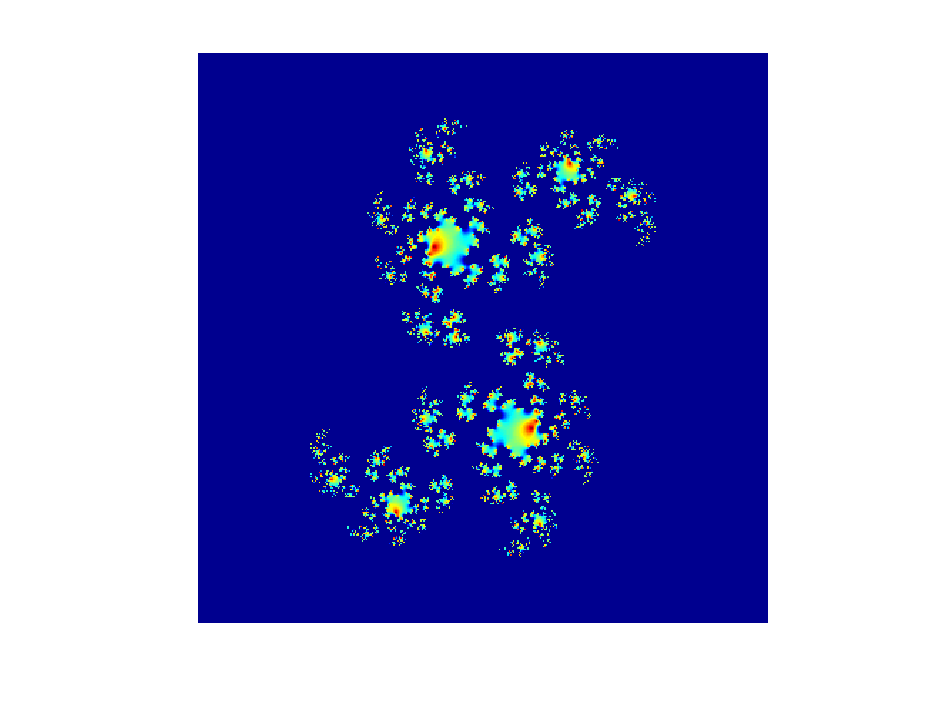
\includegraphics[scale=0.5]{julia}
\caption{We let $f(z) = z^2 + 0.4 + 0.3i$ and then iterate on a mesh from $[-1,1]\times[-i,i]$.  The above figure is a plot of $e^{-|z|}$ for each $z$ in the msh after $30$ iterations.}
\end{center}
\end{figure}


\begin{problem}
Generate another grid of complex numbers on $[-1,1]\times[-i,i]$.  Let $f(z) = z^2 + c$ where $c$ is a complex number from the mesh.  Write code that iterates each point in the mesh 30 times, and then plot $e^{-|z|}$ on the resulting mesh.  Try for several values of $c$.  You may want to use the {\tt imagesc} command for plotting your results.
\end{problem}




